\documentclass[12pt]{article}

\usepackage[pdftex]{graphicx}
\begin{document}
\title{Final Project Report : Locating Criminals Using MapReduce}
\author{Cangji Wu , Jiaran Hao, Kangyi Zhang}
\date{\today}
\maketitle

\begin{abstract}
This is our final project for the course Distributed System. To understand the design principles
of distributed system better, Our group decide to implement an application using MapReduce programming model. 
Our project emulates the situation where police intend to locate a criminal using the footage from transportation cameras. 
As the input data set could be huge and response time is valued, MapReduce is applied to solves the task distributively to
improve efficiency. In our implementation of MapReduce system, the mechanism to maintain scalability and fault tolerance is emphasized
. 
\end{abstract} 

\section {Introduction}

Our project try to help the police to build a “Criminal Positioning System”. Imagine the police want to find where the certain criminal is, what he would do?
The first step would be find a comparatively clear photo of the face of the criminal, and then using the video streams or pictures from the transportation camera or other devices of the whole town or city to find whether the criminal has shown in the specific area, if has, he might show again in the area where he has shown most of times. Then the police can send policemen to this area to wait to catch this criminal until he shows again. Figure 1 shows how to detect a human face with openCV.
We know that in computer vision technology, it is not very hard to recognize a person from the video stream or the pictures, however, this might take 1 second each picture for normal computer. To catch the criminal, we need to position the criminal as far as possible, if the police do not own a super computer, it would take several days to get the location. However, with map reduce, they can distribute the jobs to several computer to search the criminal at the same time, this would save a lot of time!

\begin{figure}[h!]
  
  \centering
    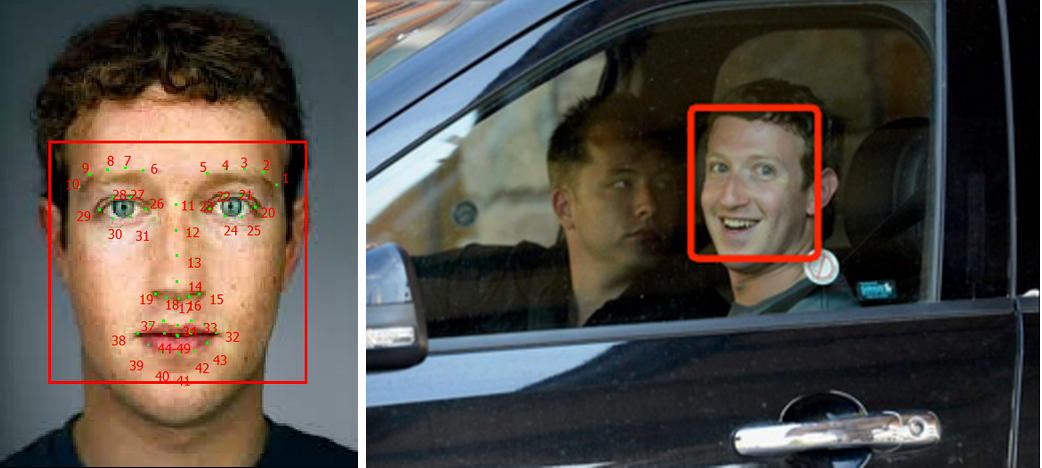
\includegraphics[width=1\textwidth]{2.png}
    \caption{Detect a human using his photo.}
\end{figure}



\section {Basic Concepts}

In our project, we do not use the real face an pictures to realize our map-reduce function, instead, we focus on how to implement the map and reduce function in our whole system.

We use C++ and OpenCV to create a lot of pictures which contains several shapes in the same picture. We have circle, triangle, rectangle to represent the real pictures from the cameras. 

\begin{figure}[h!]
  
  \centering
    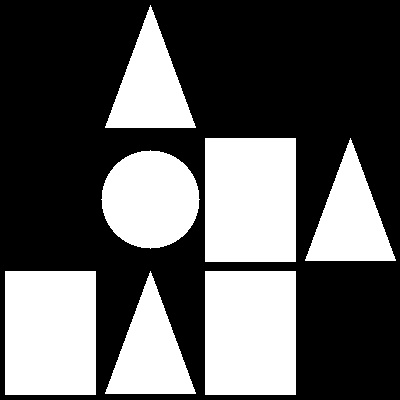
\includegraphics[width=0.5\textwidth]{1.jpg}
    \caption{Sample image of our test images.}
\end{figure}

Figure 2 shows what our images like. Suppose one of them demonstrates “criminal” and the others demonstrates “normal people”. If the circle represents our “criminal”, then our job is to find the circles from all the pictures and return the location and times of where the circle shows. In our model, master is in charge of assigning jobs to a set of workers so that workers can know when they do “Map” and when they do “Reduce”. “Map” workers are in charge of using OpenCV to find where the circle is in the pictures, “Reduce” workers are in charge of requesting the result from “Map” workers and adding them together. The file system is in charge of storing all the pictures and the result calculated from “Reduce” workers and it has the communication with the “Reduce” workers and “Master”. We will discuss their jobs in detail below.


\begin{figure}[h!]
  
  \centering
    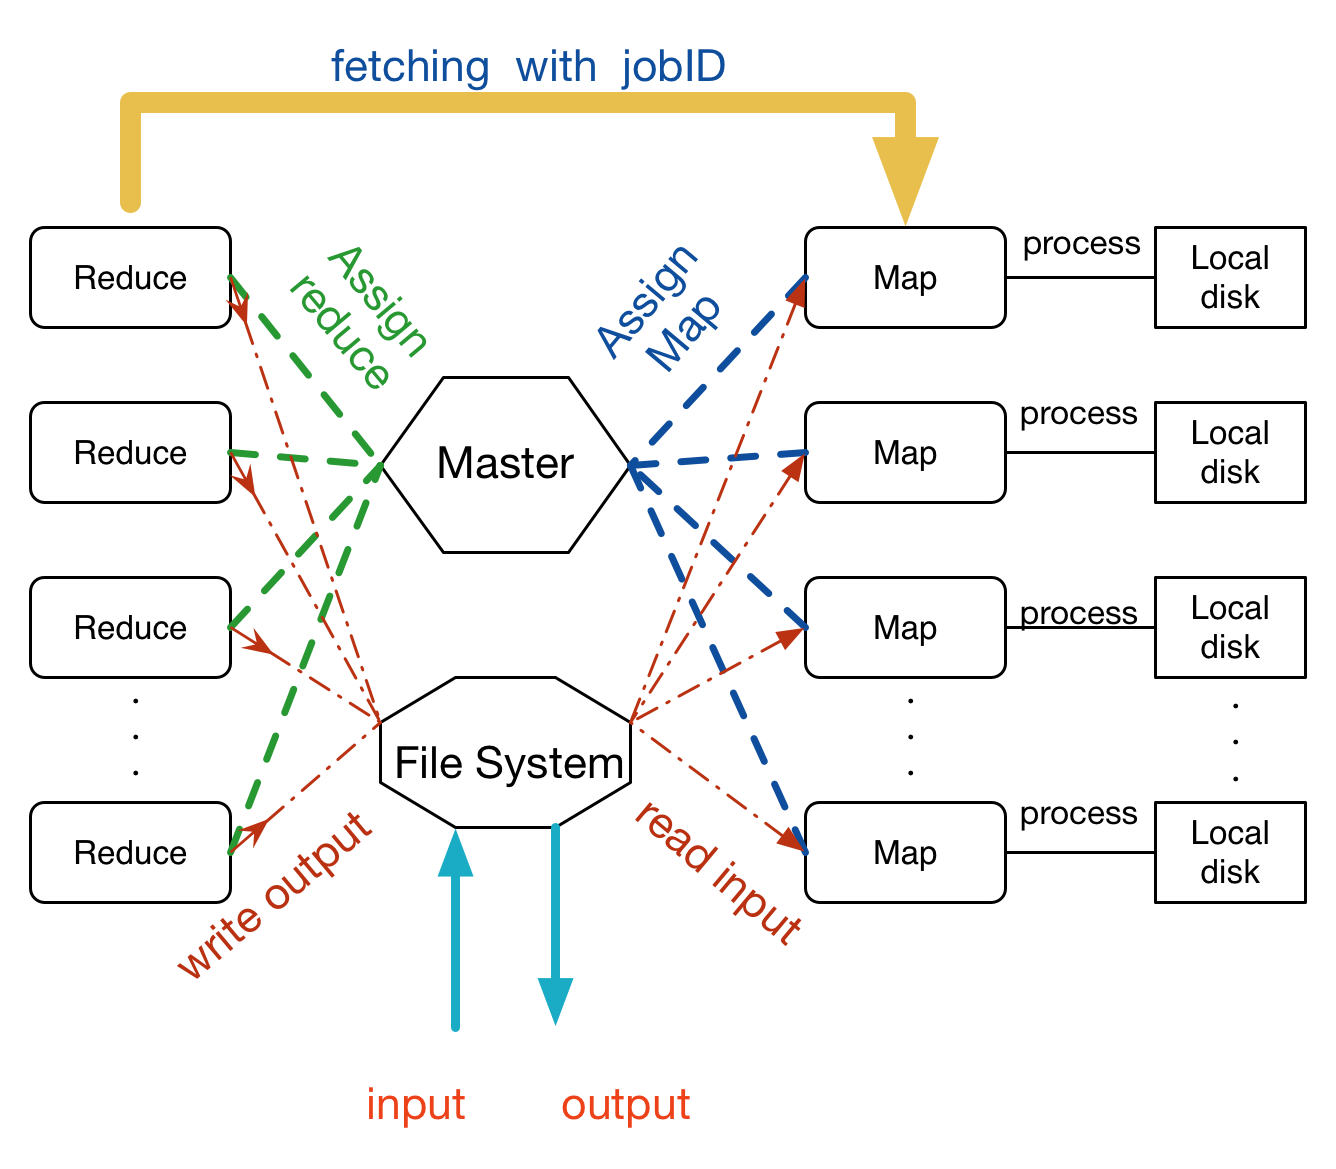
\includegraphics[width=1\textwidth]{3.png}
    \caption{Whole system.}
\end{figure}

\section {Implementation}
\subsection{Components}

In our implementation, we have five main components.  Figure 3 shows how our whole system works.
Map function and Reduce function are separated from Worker such that any Map function and Reduce function which
follows the interface can be integrated into our system.
Master and Worker are designed to manage the whole structure. In other words, they manage the communication that
is essential no matter what specific Map and Reduce function is running on the infrastructure.
File system...
Following this design, we separate our application and infrastructure so that our design is flexible enough
for any job that fits into MapReduce model. 
\subsection{Locating Algorithm }

In real situation, the images to processing would come from hundreds of cameras located in different places. And these images came from video for hours or days. So the number of images might be extremely huge, and they were stored in different places. Furthermore, the size of one image could be also very large, cause to accurately detect if this camera catch the criminal, a clearer image might be needed. Besides these, implying face recognition in just one picture to match a face with a picture of the criminal we have would also consuming a large amount of time. While to catch or monitor the criminal, the time to locate the criminal need to be as short as possible. All the reason above, which showing that using only one computer would consuming huge bandwidth, time, and other resources, push us to implementing MapReduce model in the criminal locating system, which could separate the job into several pieces and using several computers to finish this job together. 

One part of the criminal locating system is facial detection. Some facial recognition algorithms identify facial features by extracting landmarks, or features, from an image of the subject's face. For example, an algorithm may analyze the relative position, size, and/or shape of the eyes, nose, cheekbones, and jaw. These features are then used to search for other images with matching features. Other algorithms normalize a gallery of face images and then compress the face data, only saving the data in the image that is useful for face recognition. A probe image is then compared with the face data. One of the earliest successful systems is based on template matching techniques applied to a set of salient facial features, providing a sort of compressed face representation.

But in this project, image processing is not the key point. Instead we create images by ourselves, which have several simple shapes, among them we take the shape circle, as the face of criminal, and implementing circle detection instead of face recognition. And without accurate facial recognition, the number of catched circles may have some error.

In workers for map, after processing \lq\lq face recognition\rq\rq, it would building a map with location names and the frequency of appearance of criminal in that location. Then high frequency presents high probability to find the criminal, and we could start the catching action. 
\subsection{File System}
\subsection{Master}

Master manages the whole MapReduce system. It has 4 main functions: \\
First, master keeps record on who and where the workers are in a table. It holds the IP address and 
port number of each worker who participates in completing the job. The workers send \lq\lq JOIN\rq\rq\  
message to the master then master will assign a unique worker ID for the newly join worker.
Then the worker will keep sending \lq\lq UPDATE \rq\rq\ message to the master so that the master would know
if a worker has left or crashed.
  
Second, with the all the information of its workers known by the master, it will assign jobs. It will
first divides the whole input as equally as possible then assign a job ID for each job. Then master will informs the workers and tell them 
what job they account for. The jobs fall into two categories, Map and Reduce. For map worker, the master tells
them where to look for the input data on the global file system and its job ID. For Reduce worker, the master tells
them from which map workers they should fetch the intermediate results from. After assigning the jobs, the worker table
is also updated to keep track all the information so that when node fails, it can find another node to take place of the 
failed one.

Third, master also plays an important role in identifying failed workers and recovery from fault. The concrete mechanism
is discussed in the fault tolerance section.

At last, master will monitor the working state of its workers such that it will know who has completed its assigned jobs. When all 
the reduce workers complete jobs, the master will know that it is ready to output the result to the user and will notice all the map and
reduce worker to delete their temporary results and free the resources that they are holding. In addition, by keeping the status of workers,
the system can improve efficiency by transferring the jobs from heavy-loaded workers to the ones who already finish their job such that no
node will become the bottle-neck. Keeping the work load even is essential to the scalability of the system.   
\subsection{Worker}

In MapReduce model, the worker's job seems simple : if one is assigned as a map worker, it should fetch the input in the global file system and
call the Map function. Then it stores the intermediate result on local disk, waiting for the reduce worker to ask for data. The reduce worker
is even simpler. Just fetch the intermediate result from map workers, call Reduce function and write the final result to the global disk. 

However, a more efficient and fault-tolerant system requires more consideration. A worker should be designed to take more than one job. In this
way, we can transfer jobs from heavy-loaded workers to less loaded ones or reassign jobs if one node fails. In Google thesis on MapReduce, they just assume that there would always be enough workers left. While our implementation wants to make sure the system will give the correct input no matter how many nodes go down. If only one node is left, it will take all the jobs itself. This design makes sense because it first ensures correctness then allows improvement on efficiency by adding more workers.
In addition, when the reduce workers fetch intermediate data, the map workers they try to connect may already be down. If so, the reduce workers
should have the mechanism to wait for the master to inform them that they should inquire another node instead of the crashed one.

Therefore, when master assigns jobs, each job has a job ID. The reduce worker will keep a map whose key is a unique job ID and value is the contact information of relevant map node. Similarly, map workers also keep a map using job ID as the key as they may hold intermediate result of several different jobs.
    
\subsection{Fault Tolerance}

Most principle in designing distributed system is actually helping people to fight node fault. In our design, we combine three most common techniques used in the distributed systems to tolerate faults.

First, replication. Several copies of the input data are stored on different node such that if one goes down, the substitute will always have access to required input. Actually, the distributed file system itself can be a very complex component instead of our simple stimulation. The file system is a key part of the Hadoop platform.   

Second, heart beat. In our system, every node keeps update message to the master, the master has a timer to count the interval of each update message. If one node fails to send the update message for some reason, the master goes into a process to reassign jobs. It will first find the least loaded node and read the worker table to get all the jobs that are assigned to the failed node then transfer those jobs to the least loaded node. If a job is a Map job, it will also find which reduce worker is responsible for this map job and tell this reduce worker to go to the new node. Here, our job ID can be very convenient. We can just use to job ID to access the map in the reduce worker and change the value(address).
 
Note that this reassign process must reassign the reduce job first and then the map jobs. Because in our implementation a worker can have both map job and reduce job at the same time and the reduce job may wants to fetch data from the same node. If the reduce job are reassigned first, the master will inform the new node when reassigning the map job. For example, at first there are 3 nodes A,B,C and 3 jobs 1,2,3. A,B are map workers and C is reduce worker. First C goes down then master reassigns C's job(job 3) to B. Now B has one map work(job 2) and one reduce work(job 3). The reduce job(job3) says it should ask node A and node B for data. Sadly, B goes down too. At this very point, we should reassign B's job3 first thus we reassign it to A. Then we reassign B's map job(job 2), master will find A is responsible for reduce B's map job. Eventually, A has 3 jobs and finish the whole operation. Otherwise, we will fail to find who is responsible for job 2 because B is already down.

Third, logging to fight master fault. This part is not implemented in our code for time limit but is still essential to the system. When master assigns job and update each worker's status. It should keep a log in the global file system. When master goes down, we find another available worker and converts it to master. It then reads the log in the global file system then initializes according to contents in the log and keep doing the master's work.

These three techniques will defend most of the fault cases as they did in other distributed systems.
   
\subsection{Scalability and Iterator Invalidation Principle}

Certain factors can affect the scalability of a distributed system.
 
First, the master makes sure the work is divided into pieces as evenly as possible. When dealing large data input, the cost will be amortized by
workers. No node would become the bottle-neck to slow down the whole system.
 
Second, with more workers participating, the possibility of worker fault increases. However, no relationship is established between workers which means that MapReduce system can deal with massive worker fault. For example, in Chord, if one sub-network goes down, the rings would be broken if the successor buffer fails to hold enough successors. But in MapReduce model, the workers all depend on the master instead of each other. Thus, increasing number of workers will not be a problem.

Third, as the file system is also distributed, bandwidth usage when workers inquiring input data can be minimized by smart arrangement of jobs. Most of the workers will just have to read data from itself or close neighbors. This also will not be a problem. 

However, the system has a special node. The work load of master may increase linearly as more workers coming in. Though master only handles management messages, lots of threads would be created in master as concurrency is heavily used in our program to increase performance. These threads may modify the worker table and job list etc. We have to use locks to maintain thread-safe. However, locks serialize concurrent programs thus the performance is compromised. Our method to solve this is to only lock when necessary. Iterator invalidation principle would help us in this process.

1) For data structure such as list or vector, add is invalidation free if no resizing happens. Deletion will not affect the elements before the deleted one.

2) For associative data structure such as map or set, only the reference of the deleted element is invalid.

These two principles will determine how to avoid unnecessary locks. For example, if one thread adds a new node to worker table, we should lock against other threads which want to join or delete the worker table map. But it is not necessary to prevent a thread from modifying the existing element. For the thread removing nodes that fails to update , however, we should lock against modification.        
   

\section{Experiment and Performance }

We create a program to generate random pictures as input. The program takes an integer a as input and generate a pictures with format number.placename.png.  Each pictures contains random shapes generate and their sizes are different. Then we make several copies of these pictures and store them in the nodes. We run our MapReduce application and get the output which contains location and spot frequency pairs to indicate how many times the specified shape appears in the location. The application successfully generates the output in a timely manner. Then we try to crash several workers and find that the application will still obtain the expected result but with delay. The time for the master to detect fault and reassign jobs attributes to this delay.
  
\section {Conclusion}

\section*{Reference}

[1] Jeffrey Dean, Sanjay Ghemawat, MapReduce: Simplified Data Processing on Large Clusters, 2004 \\
{[2]} Xuehan Xiong, Fernando De la Torre, Supervised Descent Method and its Applications to Face Alignment, 2013\\
{[3]} Wikipedia contributors. "MapReduce." Wikipedia, The Free Encyclopedia. Wikipedia, The Free Encyclopedia, 10 Apr. 2014. Web. 14 Apr. 2014. \\
{[4]} Wikipedia contributors. "Google file system." Wikipedia, The Free Encyclopedia. Wikipedia, The Free Encyclopedia, 1 Dec. 2007. Web. 15 Apr. 2014. \\
{[5]} Wikipedia contributors. "Face recognition." Wikipedia, The Free Encyclopedia. Wikipedia, The Free Encyclopedia, 26 Apr. 2013. Web. 15 Apr. 2014.
\end{document}
